\documentclass[tikz,border=8pt]{standalone}
% Shared look for every TikZ diagram. Load with \input{../../tools/tikz-style.tex}
\usepackage[T1]{fontenc}
\usepackage{lmodern}
\renewcommand{\sfdefault}{lmr}  % diagrams use the same serif as the text
\usetikzlibrary{arrows.meta, positioning, shapes.geometric, calc, fit, backgrounds}
\definecolor{cblue}{HTML}{4C78A8}
\definecolor{corange}{HTML}{F58518}
\definecolor{cgreen}{HTML}{54A24B}
\definecolor{cred}{HTML}{E45756}
\definecolor{cpurple}{HTML}{B279A2}
\definecolor{cgrey}{HTML}{6B6B6B}
\tikzset{
  every picture/.style={font=\sffamily, line width=1.2pt},
  box/.style={draw=#1, fill=#1!12, rounded corners=4pt, align=center, inner sep=7pt, minimum height=1.1cm},
  box/.default=cgrey,
  arrow/.style={-{Stealth[length=3mm]}, draw=cgrey, line width=1.4pt},
  title/.style={font=\sffamily\bfseries\Large},
  note/.style={font=\sffamily\small, text=cgrey, align=center},
}
\AtBeginDocument{\hyphenpenalty=10000 \exhyphenpenalty=10000}

% Thrun's door world: one door, open or closed (the state). The robot can push it or do nothing (the commands) and
% has a sensor that reads "open" or "closed" and is sometimes wrong.
\definecolor{cbrown}{HTML}{9C755F}
\begin{document}
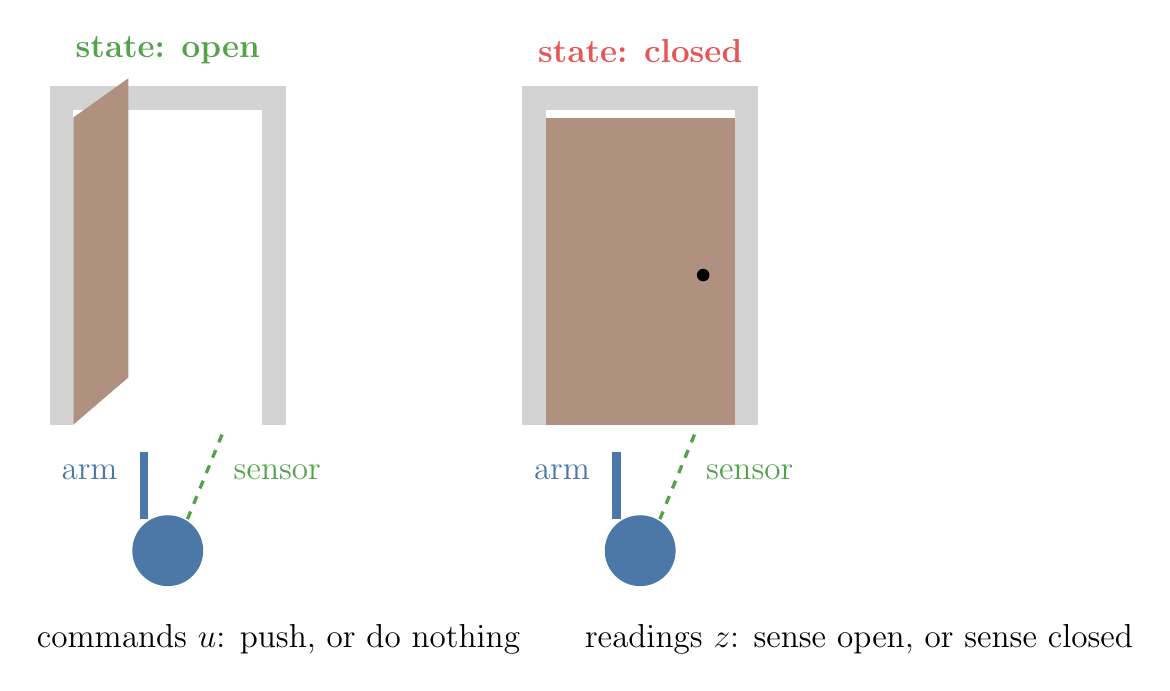
\begin{tikzpicture}[x=1cm, y=1cm, every node/.append style={font=\large}]
  \newcommand{\scene}[2]{% x offset, open (1) or closed (0)
    \begin{scope}[xshift=#1cm]
      \fill[cgrey!30] (0,0) rectangle (0.3,4); \fill[cgrey!30] (2.7,0) rectangle (3,4);
      \fill[cgrey!30] (0,4) rectangle (3,4.3);
      \ifnum#2=1
        \fill[cbrown!80] (0.3,0) -- (1.0,0.6) -- (1.0,4.4) -- (0.3,3.9) -- cycle;
        \node[cgreen, font=\large\bfseries] at (1.5,4.75) {state: open};
      \else
        \fill[cbrown!80] (0.3,0) rectangle (2.7,3.9);
        \fill[black] (2.3,1.9) circle (0.08);
        \node[cred, font=\large\bfseries] at (1.5,4.75) {state: closed};
      \fi
      % robot
      \fill[cblue] (1.5,-1.6) circle (0.45);
      \draw[cblue, line width=3pt] (1.2,-1.2) -- (1.2,-0.35);
      \node[cblue, anchor=east] at (1.0,-0.6) {arm};
      \draw[cgreen, dashed, line width=1.2pt] (1.75,-1.2) -- (2.2,-0.1);
      \node[cgreen, anchor=west] at (2.2,-0.6) {sensor};
    \end{scope}
  }
  \scene{0}{1}
  \scene{6}{0}
  \node[align=left, anchor=north west] at (-0.3,-2.4) {commands $u$: push, or do nothing\qquad readings $z$: sense open, or sense closed};
\end{tikzpicture}
\end{document}
